%!TEX root = ../NCVC.tex

\subsection{FAQ}

\subsubsection{CADデータ}

\begin{minipage}[t]{0.48\textwidth}
1) DXFデータが読めない\\
 CADで設定したレイヤ名とNCVCの読み込みレイヤ設定を合わせて下さい.
それでも読めない場合,例えば Jw\_cad の場合,
設定メニューの基本設定で[DXF書き出し]の[レイヤ名に番号を付加する]にチェックが入っていると(図\ref{fig:jw-dxf.png}),
読めない場合があります.
余分な情報が書き込まれている可能性があるので,次の項も参考に.
\end{minipage}
\begin{minipage}[t]{0.02\textwidth}
 
\end{minipage}
\begin{minipage}[t]{0.5\textwidth}
\vspace*{-2zh}
\begin{figure}[H]
\centering
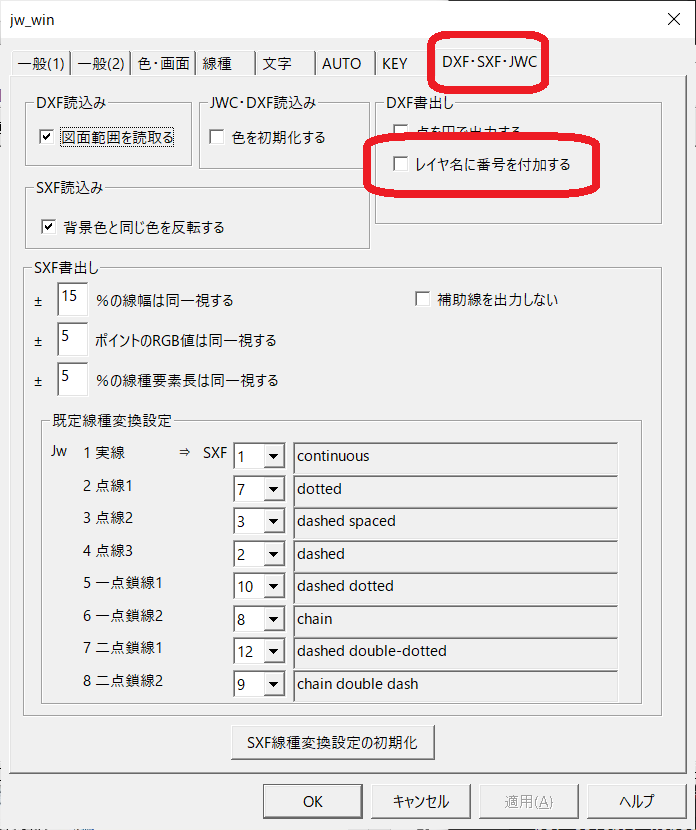
\includegraphics[width=\textwidth]{No7/fig/jw-dxf.png}
\caption{Jw\_cad の基本設定画面}
\label{fig:jw-dxf.png}
\end{figure}
\end{minipage}

\begin{minipage}[t]{0.48\textwidth}
2) CADにレイヤ名の設定がない\label{sec:ReadSetup}\\
 本来ならどうしようもないんですが...(爆)
とりあえずNCVCの読み込みレイヤ設定で正規表現を選択し[\yen{}w]と入力.
原点レイヤはそのままで,データがないときの選択をエラー以外にして下さい(図\ref{fig:ReadSetupFAQ.png}).
[\yen{}w]は正規表現の略記法で,アルファベット・数値・下線にマッチします.
この設定でDXFデータが読めれば,表示メニューからレイヤを選択し,読み込まれたレイヤ名を確認して下さい.
切削レイヤと原点レイヤの区別ができるようならその設定に合わせてあげると,以降正しく読めると思います.
\end{minipage}
\begin{minipage}[t]{0.02\textwidth}
 
\end{minipage}
\begin{minipage}[t]{0.5\textwidth}
\vspace*{-2zh}
\begin{figure}[H]
\centering
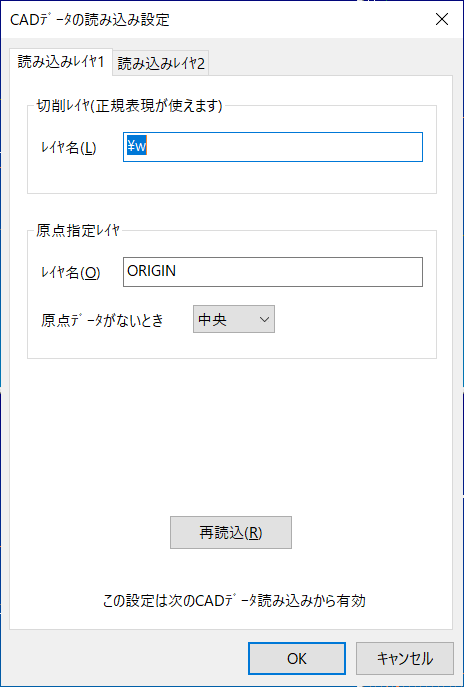
\includegraphics[width=\textwidth]{No7/fig/ReadSetupFAQ.png}
\caption{切削レイヤの特殊な読み込み設定}
\label{fig:ReadSetupFAQ.png}
\end{figure}
\end{minipage}

\vspace*{2zh}
3) それでも読めない\\
 ご使用のCADからどのようなレイヤ名で出力されているかを調査する必要がありますが,上記[\yen{}w]で読めなければ可能性は低いです.
諦めて下さい.ご使用のCADを変えましょう.

\vspace*{1zh}
4)「以下のDXFキーワード hogehoge は現在のNCVCでは未サポートです」と言われる\\
 恐らくDXFがR12形式ではありません.
読めないことはないんですがデータが欠落している可能性があるので,できるだけR12形式で保存してください.
参考までにNCVCが認識するのは
\texttt{LINE}(線),\texttt{POLYLINE}(連続線),\texttt{CIRCLE}(円),\texttt{ARC}(円弧),\texttt{ELLIPSE}(楕円),\texttt{POINT}(点),\texttt{TEXT}(文字)
の7種です.

\vspace*{1zh}
5) 3次元DXFデータはサポートされていますか?\\
 サポートされていません.
エラーにもなりませんが,NCVCはXY座標しか取得しないので正しく表示されないでしょう.
目指す所ではありますが,今のところサポートの予定はありません.

\subsubsection{Gコード生成(作図に関する注意)}

1) Z軸が途中で上昇する\\
 CADでの作図で端点が正しく接続されているか,十分拡大してもう一度確認して下さい.
Jw\_cadなら右クリック,その他のCADでも端点補助機能等を駆使し,確実に接続してください.
NCVCの加工条件,最適化タブにある「許容差」でも調整できますが,オススメできません.

\vspace*{1zh}
2) 1本の線が2つ以上のGコードに生成されている\\
 画面上で1本に見えても線が切断されていませんか?
効率が悪いので同じ傾きなら1本の線で作図しましょう.

\vspace*{1zh}
3) 同じ線を行ったり来たり\\
 画面上で1本に見えても同じ線が何本も作図されていませんか?
画面でも印刷しても解りませんが,Gコード生成では素直に生成されます.
上記も含め正しい作図を心がけましょう.

\vspace*{1zh}
4) 文字を切削したい\\
 CADで文字を入力してもコードとしか認識されません(\ref{sec:moji}節参照).
文字軌跡を切削するには文字(フォント)自体を線または円弧情報に変換する必要があります.
残念ながらNCVCにその機能は無いので,他のツールを使って変換して下さい.
ネット検索ではヒットしましたのでご参考に.市販ソフトでこの機能があることも報告されています.

\vspace*{1zh}
5) CAD図面より大きなデータを生成(加工)したい\\
 CADで図面の縮尺を指定すれば良いと思います.
ただしそのCADからDXF形式で出力したとき,実寸で出力されている必要があります.
NCVCはDXFのヘッダー情報に含まれる縮尺は無視します.
Jw\_cad では縮尺 1/100 の図面に $50\mathrm{mm}\times 50\mathrm{mm}$ の矩形を作図してNCVCで生成すると,
$5\mathrm{m}\times 5\mathrm{m}$ の矩形で生成されることを確認しています.

\vspace*{1zh}
6) NC旋盤用のGコードを生成したい\\
 残念ながらNCVCは縦フライスを前提にGコードを生成します.
旋盤用のGコードはNCVCではサポートされていません.
しかし,有志がこの問題に取り組み成果を上げています.
詳細はNCVCのWebページや掲示板を参照して下さい.

\subsubsection{NCデータ関連}

1) 拡張子なしのNCファイルが開けない\\
 現在のバージョンは[拡張子なし]が登録できません.次期バージョンで修正されています.

\vspace*{1zh}
2) NC旋盤のコードをシミュレートしたい\\
 基本的なGコードはフライス・旋盤とも同じですが,旋盤特有のコードは残念ながらNCVCではサポートされていません.
この問題も有志が取り組まれています.
詳細はNCVCのWebページや掲示板を参照して下さい.

\vspace*{1zh}
3) 工具補正が表示できない\\
 まだサポートされていません.工具補正コードは無視されます.もうしばらくお待ち下さい.

\subsubsection{システム関連他}

1) 文字化けする\\
 Windows9x系(Me含む)でNCVCを動かす,特に多数のファイルを開いたりすると,背景色が変な色になったり,メニューやダイアログの文字が化けたりする場合があります.
これは Windows 自身のリソース(資源)不足に起因するもので,以下の方法である程度は回避することができます.
\begin{itemize}
    \item 表示属性の背景色1と2を同じ色にする
\end{itemize}
 これでNCVCが使用するリソースを減らすことができます.
主に Windows9x 系のGDIリソース不足が原因で,これは本体のメモリを増設しても解決しません.
できれば Windows2000 以降での使用をオススメします.

\vspace*{1zh}
2) 外部アプリケーションでCADデータを開くには\\
 NCVCはDXF形式を読み込みますが,お使いのCAD独自形式で編集を加えたい場合,
以下のように外部アプリケーションの引数を指定すると上手く渡せます.
(AutoCAD データで編集する場合)
\begin{itemize}
    \item ``\,\$\{FilePath\}\$\{FileNameNoExt\}.dwg\,''
\end{itemize}
 ただし,当然ながら独自形式とDXF形式が同じフォルダにあって,拡張子だけが違う場合に限ります.
